%\\\///\\\///\\\///\\\///\\\///\\\///\\\///\\\///\\\///\\\///\\\///\\\///\\\///\\\///\\\///\\\///\\\///\\\///\\\///
% \\//  \\//  \\//  \\//  \\//  \\//  \\//  \\//  \\//  \\//  \\//  \\//  \\//  \\//  \\//  \\//  \\//  \\//  \\//
%  \/    \/    \/    \/    \/    \/    \/    \/    \/    \/    \/    \/    \/    \/    \/    \/    \/    \/    \/
%
%       Projekt:        Bachelor Thesis
%       Autor:          Felix Dietze
%       Datum:          2011
%
%       Comment:        Here is the definition of the titlepage
%
%  /\    /\    /\    /\    /\    /\    /\    /\    /\    /\    /\    /\    /\    /\    /\    /\    /\    /\    /\
% //\\  //\\  //\\  //\\  //\\  //\\  //\\  //\\  //\\  //\\  //\\  //\\  //\\  //\\  //\\  //\\  //\\  //\\  //\\
%///\\\///\\\///\\\///\\\///\\\///\\\///\\\///\\\///\\\///\\\///\\\///\\\///\\\///\\\///\\\///\\\///\\\///\\\///\\\

\begin{titlepage}

\begin{center}

\parbox{8cm}{
\includegraphics[height=1.6cm]{title/logo_rwth_color}}
\hfill
\parbox{2.5cm}{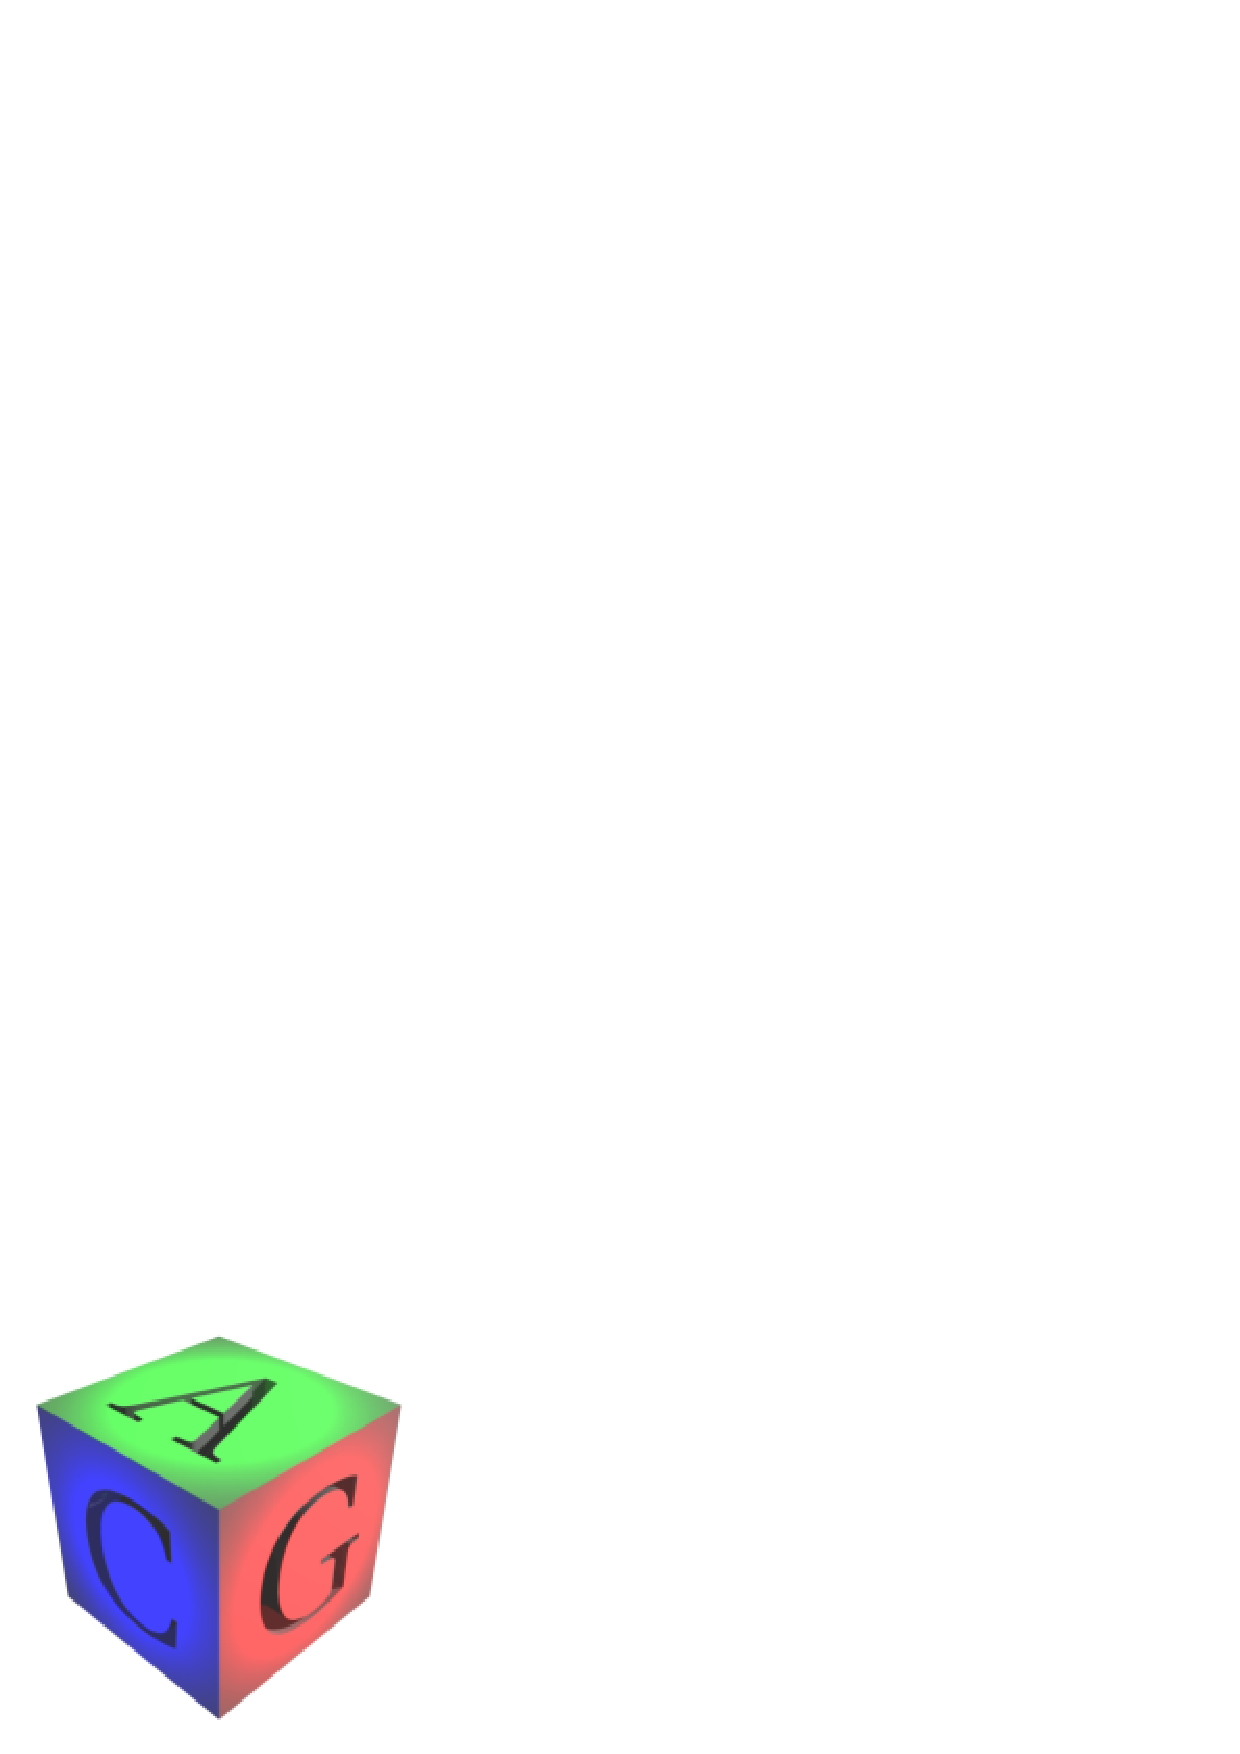
\includegraphics[width=2.3cm]{title/logo_acg_color}}

\vspace{0.5cm}

\vspace{0.75cm}

\textsf
{
Fakultät für Mathematik, Informatik und Naturwissenschaften\\
Lehrstuhl für Informatik VIII (Computergraphik und Multimedia)\\
Prof. Dr. Leif Kobbelt
}

\rule{\linewidth}{1pt}

\vspace{1.75cm}
\LARGE
\textbf{Bachelorarbeit}

\vspace{1.7cm}
\huge
Vorhersage und Interaktive Komposition von Noise-Funktionen zum Rendern Unbeschränkter Prozeduraler Welten in Echtzeit

\vspace{2.0cm}
\Large
Felix Dietze\\
\large
Matrikelnummer: 290734

\vspace{0.5cm}
August 2011

\vspace{1.05cm}
\rule{\linewidth}{1pt}

\vspace{0.5cm}
\textsf{\textbf{
\normalsize
\begin{tabular}{ll}
Erstgutachter:  & Prof. Dr. Leif Kobbelt\\
Zweitgutachter: & xxxxxxxxxxxxx\\
\end{tabular}
}}
\end{center}

\end{titlepage}
